% XCircuit output "schema_sim_C1ekvC5.tex" for LaTeX input from schema_sim_C1ekvC5.ps
\def\putbox#1#2#3#4{\makebox[0in][l]{\makebox[#1][l]{}\raisebox{\baselineskip}[0in][0in]{\raisebox{#2}[0in][0in]{\scalebox{#3}{#4}}}}}
\def\rightbox#1{\makebox[0in][r]{#1}}
\def\centbox#1{\makebox[0in]{#1}}
\def\topbox#1{\raisebox{-0.60\baselineskip}[0in][0in]{#1}}
\def\midbox#1{\raisebox{-0.20\baselineskip}[0in][0in]{#1}}
   \scalebox{0.8}{
   \normalsize
   \parbox{7in}{
   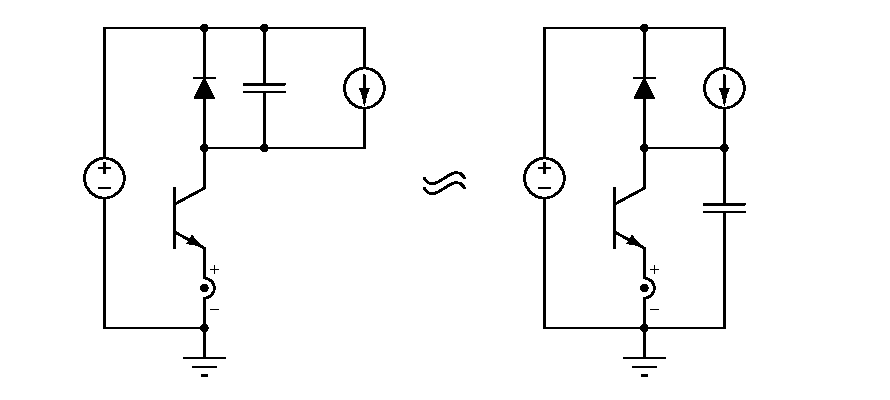
\includegraphics[scale=1.25]{schema_sim_C1ekvC5}\\
   % translate x=47 y=539 scale 0.30
   \putbox{6.11in}{1.40in}{1.20}{$C_{par}$}%
   \putbox{2.27in}{2.40in}{1.20}{$C_{par}$}%
   \putbox{0.06in}{1.29in}{1.20}{$$}%
   } % close 'parbox'
   } % close 'scalebox'
   \vspace{-\baselineskip} % this is not necessary, but looks better
